\documentclass[usenatbib]{mn2e} 
\usepackage{amsmath} 
\usepackage{amssymb} 
\usepackage{graphics}
\usepackage{graphicx}
\usepackage{epsfig} 
\usepackage{float} 
\def\be{\begin{equation}}
\def\ee{\end{equation}}
\def\ba{\begin{eqnarray}}
\def\ea{\end{eqnarray}}
\bibliographystyle{mn2e}
% To highlight comments 
\usepackage{color}
\definecolor{red}{rgb}{1,0.0,0.0}
\newcommand{\red}{\color{red}}
\definecolor{blue}{rgb}{0.1,0.3,0.9}
\newcommand{\blue}{\color{blue}}

\usepackage[normalem]{ulem}
\definecolor{darkgreen}{rgb}{0.0,0.5,0.0}
\newcommand{\SRK}[1]{\textcolor{darkgreen}{\bf SRK: \textit{#1}}}
\newcommand{\SRKED}[1]{\textcolor{darkgreen}{\bf #1}}
\newcommand{\LCDM}{$\Lambda$CDM~}
\newcommand{\beq}{\begin{eqnarray}}  
\newcommand{\eeq}{\end{eqnarray}}  
\newcommand{\zz}{$z\sim 3$} 
\newcommand{\apj}{ApJ}  
\newcommand{\apjs}{ApJS}  
\newcommand{\apjl}{ApJL}  
\newcommand{\aj}{AJ}  
\newcommand{\mnras}{MNRAS}  
\newcommand{\mnrassub}{MNRAS accepted}  
\newcommand{\aap}{A\&A}  
\newcommand{\aaps}{A\&AS}  
\newcommand{\araa}{ARA\&A}  
\newcommand{\nat}{Nature}  
\newcommand{\physrep}{PhR}
\newcommand{\pasp}{PASP}    
\newcommand{\pasj}{PASJ}    
\newcommand{\avg}[1]{\langle{#1}\rangle}  
\newcommand{\nscatt}{\langle N_{\rm  scatt}\rangle}
\newcommand{\ly}{{\ifmmode{{\rm Ly}\alpha~}\else{Ly$\alpha$~}\fi}}
\newcommand{\hMpc}{{\ifmmode{h^{-1}{\rm Mpc}}\else{$h^{-1}$Mpc }\fi}}   
\newcommand{\hGpc}{{\ifmmode{h^{-1}{\rm Gpc}}\else{$h^{-1}$Gpc }\fi}}   
\newcommand{\hmpc}{{\ifmmode{h^{-1}{\rm Mpc}}\else{$h^{-1}$Mpc }\fi}}  
\newcommand{\hkpc}{{\ifmmode{h^{-1}{\rm kpc}}\else{$h^{-1}$kpc }\fi}}  
\newcommand{\hMsun}{{\ifmmode{h^{-1}{\rm
        {M_{\odot}}}}\else{$h^{-1}{\rm{M_{\odot}}}$}\fi}}   
\newcommand{\hmsun}{{\ifmmode{h^{-1}{\rm
        {M_{\odot}}}}\else{$h^{-1}{\rm{M_{\odot}}}$}\fi}}   
\newcommand{\Msun}{{\ifmmode{{\rm {M_{\odot}}}}\else{${\rm{M_{\odot}}}$}\fi}}  
\newcommand{\msun}{{\ifmmode{{\rm {M_{\odot}}}}\else{${\rm{M_{\odot}}}$}\fi}}  
\newcommand{\lya}{{Lyman$\alpha$~}}
\newcommand{\clara}{{\texttt{CLARA}}~}
\newcommand{\rand}{{\ifmmode{{\mathcal{R}}}\else{${\mathcal{R}}$ }\fi}}  
\newcommand{\hs}{{\hspace{1mm}}}  
\newcommand{\kms}{{\ifmmode{{\mathrm{\,km\ s}^{-1}}}\else{\,km~s$^{-1}$}\fi}}

% definition to produce a "less than or similar to" symbol
\def\lsim{~\rlap{$<$}{\lower 1.0ex\hbox{$\sim$}}}

% definition to produce a "greater than or similar to" symbol
\def\gsim{~\rlap{$>$}{\lower 1.0ex\hbox{$\sim$}}}

\begin{document}

\title[Rotation in the Lyman-$\alpha$ line]{Rotation effects on the
  Lyman-$\alpha$ line morphology in distant galaxies}
\author[Garavito-Camargo, Forero-Romero \& Dijkstra]{
\parbox[t]{\textwidth}{\raggedright 
  Nicolas Garavito-Camargo$^{1}$,
  Jaime E. Forero-Romero$^{1}$ and 
  Mark Dijkstra$^2$
}
\vspace*{6pt}\\
$^{1}$Departamento de F\'{i}sica, Universidad de los Andes, Cra. 1
No. 18A-10, Edificio Ip, Bogot\'a, Colombia \\
$^2$
}
\maketitle

\begin{abstract}
Rotation is present in the gas kinematics of galaxies up to the
highest redshifts. In this paper we present for the first time
radiative transfer calculations that show the impact of rotation on
the morphology of the Lyman $\alpha$ line. To this end we construct
simplified models where a galaxy is modeled as an homogeneous sphere
composed as an homogeneous mixture of dust and hydrogen at a constant
temperature. These spheres have a solid-body rotation with linear
velocities at the surface in the range $0-300$ \kms. We consider
radiation sources both in the center of the rotating cloud and also
homogeneously distributed around the sphere. We find that higher
rotational velocities increase the width of each peak in the outgoing
line profile while it also increases the amount of Lyman alpha photons
escaping in the line center. This trends makes that for high
rotational velocities and large Hydrogen optical depths the double
peak of the line tends to be erased an be replaced by a single peak the
lines center. This is more pronounced for radiation sources
homogeneously distributed. Concerning the escape fraction we find that
rotation does not have any effect, provided that all the sources are
centrally emitted. However in the case of homogeneously emitted
sources we measure an increase of about a factor of $2$ in the escape
fraction for higher rotational velocity values. 
Our work shows clearly that gas rotation has a non negligible impact
on the shape of the Lyman $\alpha$ line. 
\end{abstract}
\begin{keywords}
galaxies: high-redshift - galaxies: star formation - line: formation
\end{keywords}


\section{Introduction}
\label{sec:intro}



Due to the resonant nature of the Lyman alpha line, gas kinematics
play an important role shaping its morphology...

There is an extensive literature studying the influence of
outflow/inflow configurations in the shape of the outgoing Lyman-alpha
line...

In this paper we study for the first time the impact of rotation on
the morphology of the Lyman $\alpha$ line. To isolate the effects of
rotation we focus on a simple system: the gas distribution is
spherical, with homogeneous density and the gas rotates as a solid
body. We base our work on two independent Monte Carlo based radiative
transfer codes CLARA \citep{CLARA} and XX \citep{DijkstraKramer}.

 
This paper is paper is structured as follows...

In this paper we express a photon's frequency in terms of the
dimensionless variable $x\equiv (\nu -\nu_a)/\Delta\nu_\alpha$, where
$\nu_{\alpha}=2.46\times 10^{15}$ Hz is the Ly$\alpha$ resonance
frequency,  $\Delta_{\alpha} \equiv
\nu_{\alpha}\sqrt{2kT/m_pc^2}\equiv \nu_av_{\rm th} $ is the doppler
broadening of the line which depends on the neutral gas temperature
$T$ scattering the radiation or equivalently the thermal velocity
$v_{\rm th}$ of the atoms.


\section{Modeling Bulk Gas Rotation}
\label{sec:implementation}

Describing the kinematics of gas rotation in all generality is a
complex task. There is great variation in the shape of the rotation
curve as observed in HI emission as a function of the distance to the
galaxy center. However there are two features that are observed very
often. First, in the central region the velocity increases
proportional to the radius following the behaviour in a body with
solid rotation. Second, beyond a certain radius the rotation curve
tends to flatten. Furthermore, a thorough observational account of gas
rotation in the redshifts of interest for the study of LAEs ($z>1.0$)
is still missing. 


An ab-initio description of realistic rotation curves in simulations
depends on having access to the dynamic evolution the mass components
in the galaxy: stars, gas and dark matter. Such level of realism is
extremely complex to achieve, specially of one wants to get a
systematic description based on statistics of simulated objects.


Following the tradition of studies of Lyman$\alpha$ emitting systems,
we implement a model with a simplified geometry and gas
distribution. We assume that the gas is homogeneously distributed in a
sphere that rotates as a solid body with constant angular
velocity. This simple model will contain only one parameter: the
linear velocity at the sphere's surface, $V_{\rm max}$.

\subsection{Detailed Implementation of Rotation}

 In the MonteCarlo code we define a cartesian coordinate system to
 define the position of each photon. The origin of this system
 coincides with the center of the sphere and the rotation axis is defined
 to be $z$-axis. With this choice, the components of the gas bulk velocity
 field, $\vec{v} = v_{x}\hat{i} + v_{y}\hat{j} + v_{z}\hat{k}$, can be
 written as  
  
\begin{subequations}
\begin{align}
    v_{x}=-\dfrac{y}{R}V_{\rm max}, \label{subeq1}\\
    v_{y}=\dfrac{x}{R}V_{\rm max}, \label{subeq2}\\
    v_{z}=0, \label{subeq3}
\end{align}
\end{subequations}
%
where $R$ is the radius of the sphere and $V_{\rm max}$ is the linear
velocity at the sphere's surface. The minus/plus sign in the
$x$/$y$-component of the velocity indicates the direction of
rotation. In this case we take the angular velocity in the same
direction as the $\hat{k}$ unit vector. With these definitions we can
write the angular velocity as $\omega=V_{\rm max}/R$.  

In contrast with spherically symmetric models (static, outflow,
inflow) the rotation now defines a preferred direction in the
problem. In Section \ref{sec:results} we quantify this differences by
varying the line of sight of a mock observer with respect to the
rotation axis. The results are parametrized by the polar angle
$\theta$ as defined by the dot product $\cos\theta =
{\hat{u}\cdot\hat{k}}$. 

\subsection{Grid of Simulated Galaxies}
\label{sec:models}

In the Monte Carlo calculations we follow the propagation of $N_{\gamma}=10^5$
numerical photons through different spherical galaxies, each one
varying in at least one of the following parameters: the maximum
rotational velocity $V_{\rm max}$, hydrogen optical depth $\tau_{H}$,
dust optical depth $\tau_{a}$ and the initial distribution of photons
with respect to the gas. There are in total 60 models with the input
parameters summarized in Table \ref{table:models}.  

\begin{table}
\begin{center}
\begin{tabular}{llc}\hline\hline
Physical Parameter (units) & Symbol & Values\\\hline
Velocity (\kms) & $V_{\rm max}$&$0,\ 50,\ 100,\ 200,\ 300$\\
Hydrogen Optical Depth & $\tau_{H} $ & $10^{5},\ 10^{6},\ 10^{7}$\\
Dust Optical Depth & $\tau_{a}$ & $0$,$1$\\
Photons Distributions & & Central, Homogeneous\\\hline\hline
\end{tabular}
\caption{
List of the physical parameters that define the spherical models we
have simulated using Monte Carlo calculations. For each parameter we
vary the values in the range listed in the last column. Takig into
account all the possible combinations we end up with $60$ different
models. } 
\label{table:models}
\end{center}
\end{table}


\section{Results}
\label{sec:results}

\begin{figure*}
  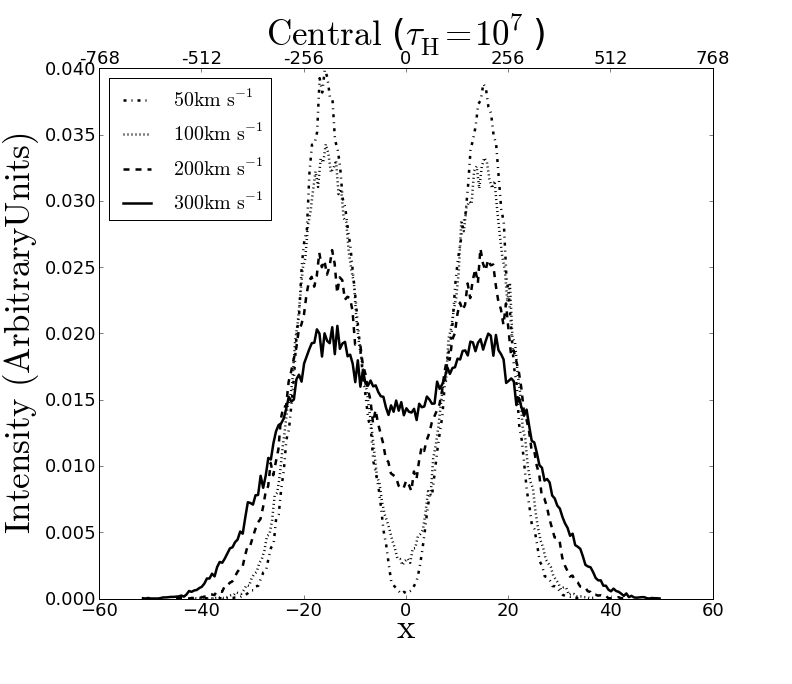
\includegraphics[width=0.45\textwidth]{SpectraDifVelocitiesCentral.png}
  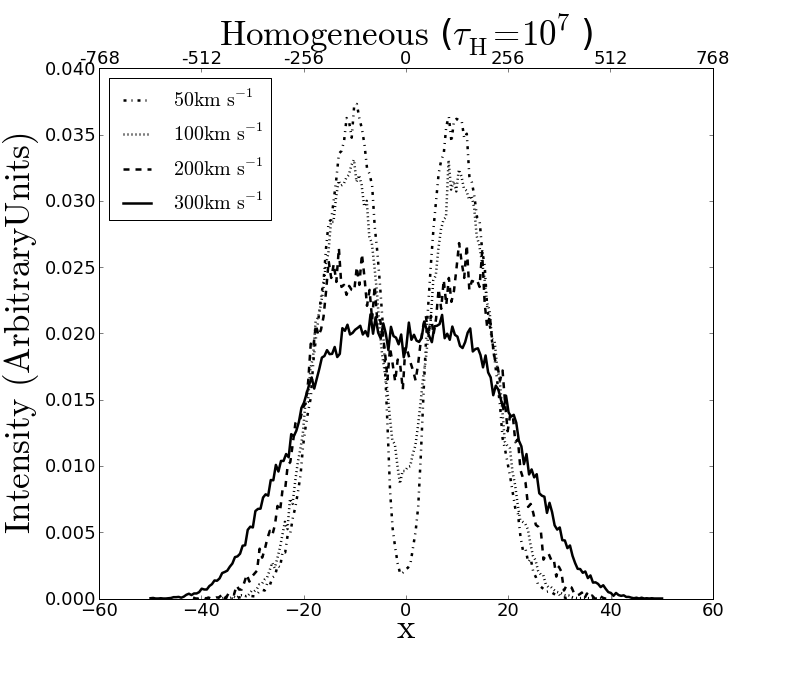
\includegraphics[width=0.45\textwidth]{SpectraDifVelocitiesHOM.png}
\caption{Shape of the \ly line for
    different velocities rotational velocities for spherical
    distributions with $\tau_{H}=10^{7}$. The left (right) panel shows
    the central    (homogeneous) photon distribution. All photons were
    taken into     account regardless of their propagation
    direction.    \label{fig:differentvelocities}}  
\end{figure*}


The central result of this paper is summarized in
Fig.~\ref{fig:differentvelocities} that shows clearly the considerable
impact of rotation on the morphology of the emergent \ly line. Both
panels in the Figure focus on the results for $\tau_{H}=10^{7}$,
showing that the influence of rotation is present both when the
photons are either homogeneously or centrally initialized over the gas
volume. 

In the following subsections we characterize the line morphology by
the half-width at half intensity and the peak maxima. In order to
interpret the morphological changes in the line we also report the
median number of scatter for each \ly photon in the
simulation. Finally we measure the bulk escape fraction as a function
of rotational velocity in the presence of dust.


All the results in this section are constructed by taking into
account all outgoing photons regardless of the direction of
propagation. In the next section \ref{subsec:direction} we quantify 
the changes in the observed spectra for observers with different
viewing angles. 

\subsection{Line width and peak maxima}
\label{sec:widthpeak}


\begin{figure}
    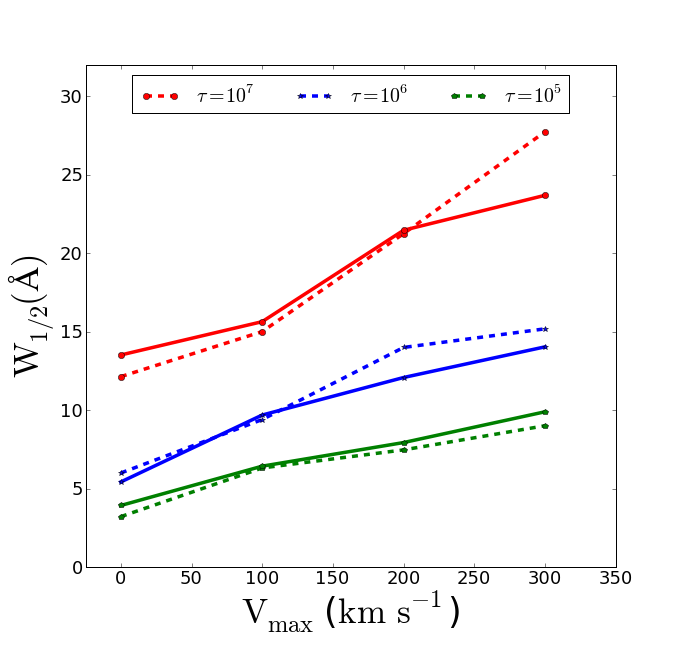
\includegraphics[width=0.45\textwidth]{WidthvsVmax.png}
    \caption{Half-width for the non-dusty models as a function of
      rotational velocity $V_{\rm max}$. Continuous (dashed) lines
      correspond to homogeneous (central) source
      distributions. \label{fig:widthvsvelocity}} 
\end{figure}


\begin{figure}
    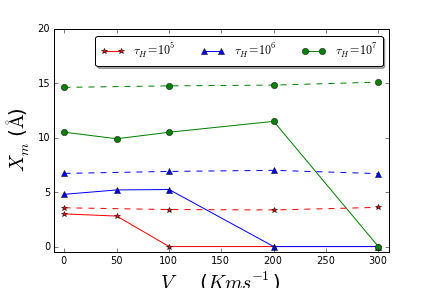
\includegraphics[width=0.45\textwidth]{maximumvsVmax.png}
\caption{Position of the peak maxima as a function of rotational
  velocity $V_{\rm max}$. Continuous (dashed) lines correspond to
  homogeneous (central) source distributions. A value of $x_{\rm
    max}=0$ indicates that line becomes single
  peaked. \label{fig:maximumsvsvelocity}}  
\end{figure}

The first quantitative conclusion of the effect of rotation in the
\ly line is that double peaks broaden and reduce their intensity
while the line center rises. This produces the impression that, as the
rotational velocity increases, the double peaks are merged into a
single broad emission peak. This is most evident in the highest
rotational velocities for the homogeneously distributed sources
(right panel in Fig.~\ref{fig:differentvelocities}). 

To quantify the line broadening we measure a modified version of the full
width at half maximum (FWHM). Instead we measure it only for half of
the line, $W_{1/2}$. This definition allows us to quantify the line
width both in the cases of double and single peak emission.  In the
case of double peaked emission $W_{1/2}$ corresponds to the width of a
single peak, while in the extreme case of high rotational velocities,
when the double peak is erased, it simply correspond to half FWHM.  

Figure \ref{fig:widthvsvelocity} shows how $W_{1/2}$ increases with
rotational velocity. Continuous (dashed) lines connect the results for
homogeneous (central) source distribution. The line width increases
with rotational velocity up to factors of $\sim 2$ at $300$\kms with
respect to the static case. For the temperature $T=10^4$K used in our
radiative transfer calculations calculations the thermal velocity is
$v_{th}=12.8$\kms. For a model with $\tau_{H}$ it means that the
half-width can increase up to $350$\kms (at $V_{\rm max}=300$\kms)
compared to a half-width of $150$\kms in the static case.  




Figure \ref{fig:maximumsvsvelocity} shows the position for the peak
maxima as a function of the rotational velocity $V_{\rm max}$. This
figure shows us clearly that in the case of central distributed
sources there is barely any change with rotational velocity in the
range of explored parameters. However, in the case of
homogeneously emitted sources the maxima position remain close to
constant until beyond some velocity threshold the line becomes single
peaked with $x_{\rm max}=0$. 

It is probable that the transition to a single peak line occurs for systems
where it  becomes easier for the bulk of the photons to escape with the lowest
number of scatterings possible, allowing them not to move very far
from the center of the line. This hypothesis can help to explain how the
single peak stage is easily achieved in the homogeneous source
distribution. In this case there is a fraction of the photons that are
inside a photosphere region with $\tau_{H,r}\ll \tau_{H}$ where
$\tau_{H,r}$ is the optical depth from the radius of emission to the
sphere's surface. This conditions allows the photons to escape with
much less scatterings compared to the photons emitted at the very
center of the sphere. In turn, it gives the photons less scatterings
to be placed far from the line center. Increasing the rotational
velocity $V_{\rm max}$ reduces the optical depth making the
photosphere region effectively larger, increasing the number of
photons escaping close to the lines's center. For the central case the
photosphere is not present, and other mechanisms must be at play in
the steady reduction of the double peak. 

For larger values of $\tau_{H}$ the transitional velocity $V_{\rm
  trans}$ is also larger. In our models we find the following
correspondence between the optical depth $\tau_{\rm H}=\{10^5, 10^6,
10^7\}$ and the transitional velocities $V_{\rm
  trans}=\{50-100\kms, 100-200\kms, 200-300\kms\}$ which can only be
constrained to be in the range of velocities in the models that gave a $x_{\rm
  max}\neq 0$ and $x_{\rm max}=0$.   In the next section explore the
origin of this trends and consider to what extent the hypothesis of a low
number of scatterings is correlated with the emergence of a single
peak. 



\subsection{Average Number of Scatterings}


\begin{figure}
    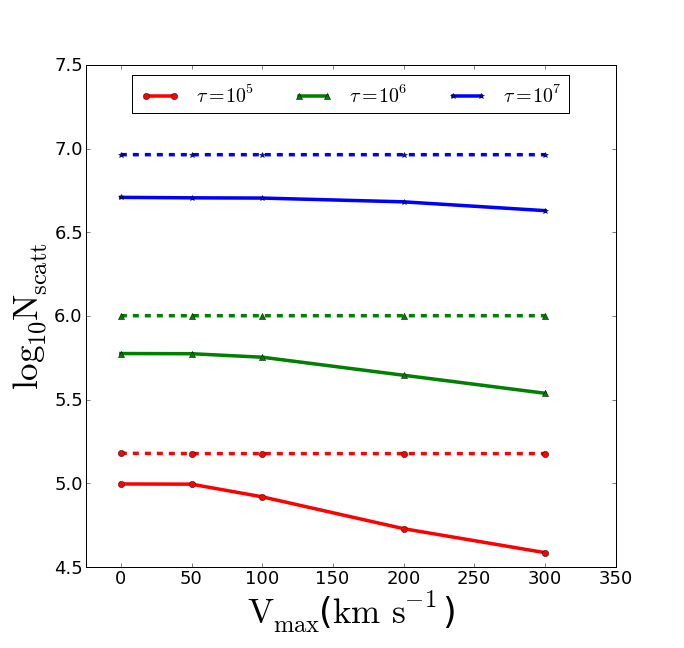
\includegraphics[width=0.45\textwidth]{NscattvsVmax.png}
\caption{Logarithm of the average number of scatterings as function of
  the velocity. \label{fig:Nscatt}}   
\end{figure}


\begin{figure*}
     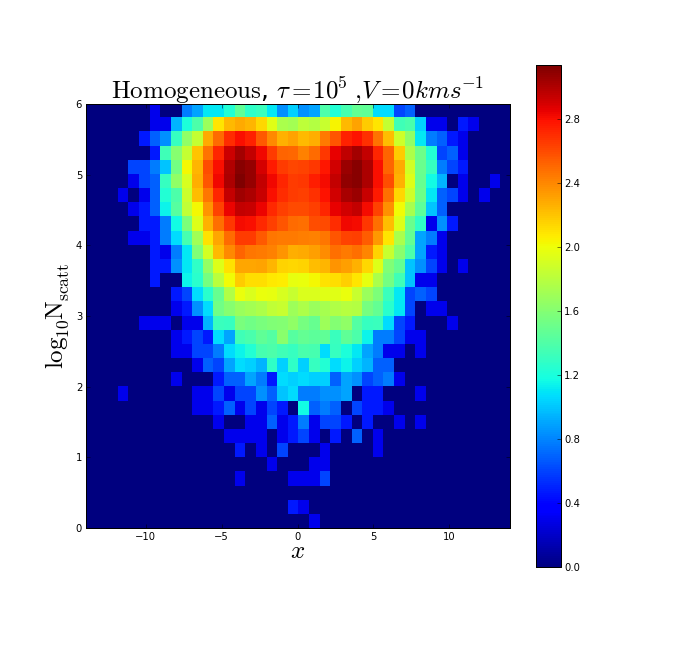
\includegraphics[width=0.45\textwidth]{2dHistogram0t5HOM.png}
     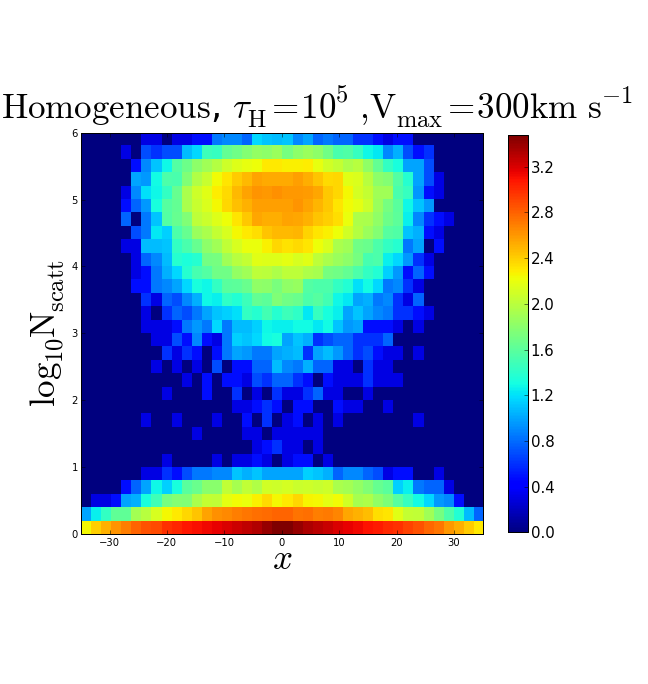
\includegraphics[width=0.45\textwidth]{2dHistogram300t5HOM.png} 
     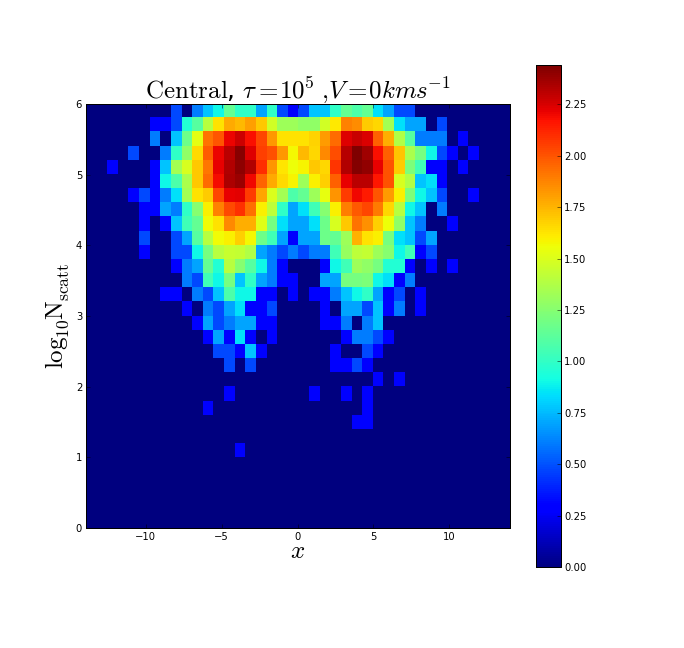
\includegraphics[width=0.45\textwidth]{2dHistogram0t5.png}
     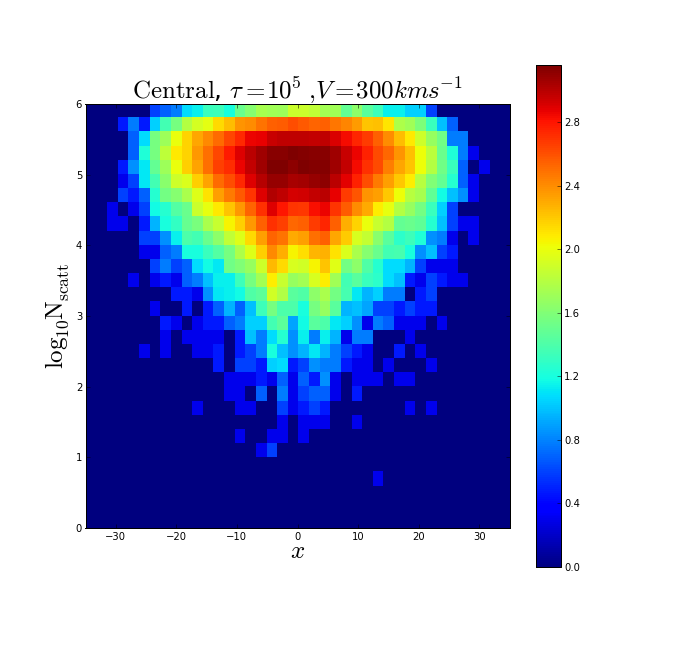
\includegraphics[width=0.45\textwidth]{2dHistogram300t5.png}    

    \caption{2D histogram of $N_{scatt}$ vs $x$. The upper (lower) pannels
      show the homogeneous (central) source distribution. Left
      corresponds to the static case and the right
      $V_{max}=300km/s$. The colour scale is locarithmic\label{fig:Nscatt2D}}  
\end{figure*}



The number of times that a \ly photon is absorbed and re-emitted is
connected to the final frequency that it can have after escaping the
galaxy. In the case of static gas geometries, a large value of the
optical depth is immediately followed by a high number of
scatterings. In turn a large optical depth increases the probability
that a \lya photon will be found far from the center of the line. The
peak maxima shifting away form the line center as the amount of
neutral hydrogen increases.


In Figure \ref{fig:Nscatt} we see the average number of scatterings
$\langle N_{\rm scatt}\rangle$ as a function of the rotational velocity
$V_{\rm max}$. For the central distributions we find that there is not
a significant change for increasing rotational
velocities, $\langle N_{\rm scatt}\rangle$ changes less than $0.5\%$
for different velocities. In this case we also find that the average
number of scatterings is proportional to the optical depth, as
expected in analogy from the analytic result for the homogeneous
infinite-slab $\langle N_{\rm  scatt}\rangle=1.612\tau_{\rm   H}$
\citep{Adams72,Harrington73}. In our experiments we find  $\langle N_{\rm
  scatt}\rangle= XXX\tau_{\rm   H}$. 


However, for the homogeneous distribution there is a clear decrease of
$\langle N_{\rm  scatt}\rangle$ as the  $V_{\rm max}$ increases. This
effect more pronounced for the lower values of the optical depth. For
$\tau_{\rm H}=10^5$ the average number of scatterings decreases by
$XX\%$ at $V_{\rm max}=300\kms$ in comparison to the static case.


The analytic expectation for the slab with homogeneously emitted
sources is $\langle N_{\rm  scatt}\rangle=1.16\tau_{\rm   H}$
\citep{Harrington73}, a factor of $0.72$ lower than the case of the
centrally emitted photons. In our case we find that for the static
spheres this factor is $xxxx$.

In order to gain a deeper understanding of these results we prepare 2D
histograms for the number of scatterings as a function of the outgoing
dimensionless frequency $x$. In Figure \ref{fig:Nscatt2D} we show
the results of such histogram in the case $\tau{\rm H}=10^5$ for the
static case and $V_{\rm max}=300$\kms. The upper (lower) panels show the
results for the homogeneous (central) source distribution. The color
scale is logarithmic in the number of photons at a certain value
$x-N_{\rm scatt}$. This Figure clearly support our hypothesis about
the photosphere in the homogeneous distribution, in this case most of
the photons that left with $x\sim 0$ have escaped with less than $10$
scatterings, clearly explaining the origin of a single central
peak. However, for a central distribution the situation is
different. In this case the number of scatterings remains high, on the
order of the optical depth, but the two peaks do get closer to each
other. In this situation each scattering leaves the photon closer to
the center of the line than the static case.

\subsection{Dusty Clouds: Escape Fraction}
\label{sec:escapefraction}


\begin{figure}
  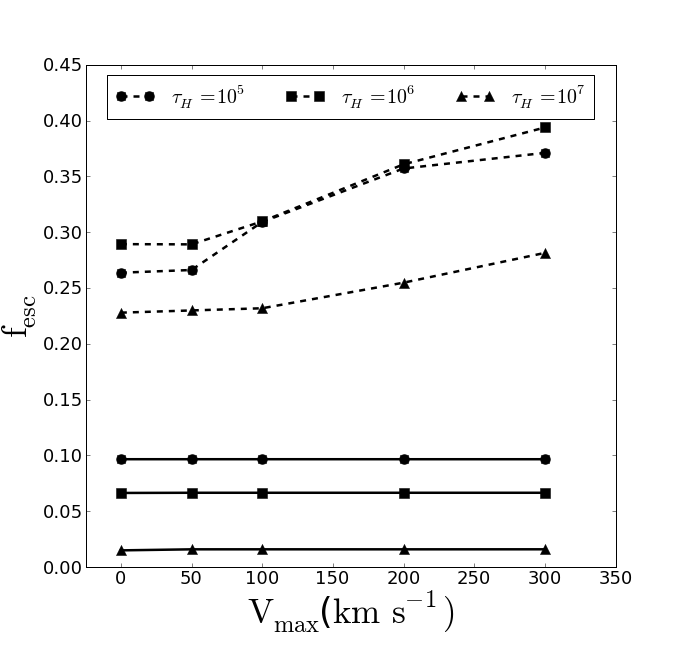
\includegraphics[width=0.45\textwidth]{escapefraction.png}
   \caption{Escape fraction as a function of rotational velocity. The
     continuous (dashed) lines correspond to homogeneous (central)
     models.
     \label{fig:efvsv}}
\end{figure}


\begin{figure}
  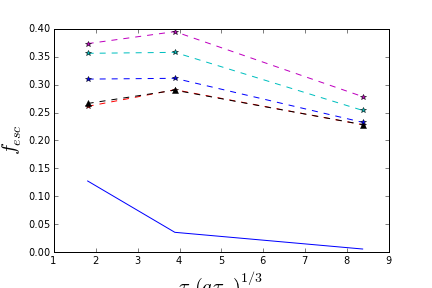
\includegraphics[width=0.45\textwidth]{Neufeld.png}
 \label{fig:efvsNeufeld}\caption{Escape fraction as a function of the
   product $(a\tau_{\rm H})^{1/3}\tau_{a}$. The analytic solution for
   the infinite is slab shown as a continuous line. Different dashed
   lines correspond to different rotational velocities.}   
\end{figure}

We also study a dusty cloud configuration to measure the effect of
rotation on the escape fraction. We expect that the modified number of
scatterings to be reflected in this amount of photons absorbed by
dust. Following this line of thought,  we do not expect any change in
for a dusty cloud with central source of radiation given that the
number of scatterings remains close to constant. On the other hand, in
the case of an homogeneous radiation source the number of scatterings
drops as $V_{\rm max}$ increases, which might be reflected as an
increasing escape fraction.

%If there is a change in the number of scatterings with rotational
%velocity, there must be a change in the probability of being absorbed
%if dust is present. We study how rotation impacts the escape fraction
%of \ly photons. 

%Taking into account the results in the previous section, we do not expect any
%change in the case of central distributions given that the average
%number of scatterings remain constant. On the other hand, in the
%homogeneous distribution there is a considerable drop in the number of
%scatterings as $V_{\rm max}$ increases, this preconditions the escape
%fraction to increase as well.

Figure \ref{fig:efvsv} shows the dependence of the escape fraction as
a function of the maximum rotational velocity, confirming that our
intuitions in this respect is correct. For the central source
distribution the escape fraction barely shows any change, while for
the homogeneous case there is a clear rise in the escape fraction for
high rotational velocities.  Rotation has a higher relative impact in
the models with low optical depth $\tau_{\rm H}=10^5$,$10^{6}$, where
it can raise from $xxx$ in the static case up to $xxx$ at $V_{\rm
  rot}=300$\kms. 


%This Figure illustrates how our
%reasoning in the previous paragraph is correct. 
%The escape fraction
%barely changes for the central source distribution, while it rises
%as the velocity $V_{\rm max}$ increases for the homogeneous case. 


In Figure \ref{fig:efvsNeufeld} we put these results in the context of
the analytical solution for the infinite slab \citep{Neufeld90}. In
Neufeld's setup the analytic solution depends solely on the product
$(a\tau_{\rm   H})^{1/3}\tau_{a}$, an approximation that is valid only
in the limits $a\tau_{\rm   H}\gg 1$. The dashed lines in Figure
\ref{fig:efvsNeufeld} correspond to the cases of different
velocities. We observe that the escape fraction is higher
by factors of $2-10$  than the expected values for the slab
configuration. We also see that for the lower value $\tau_{\rm
  H}=10^{5}$ the escape fraction does not increase with respect to the
solution for $\tau_{\rm H}=10^{6}$ as expected, however we not that we
are in a regime where the condition for the analytic expectations 
($a\tau_{h}\gg 1$) does not hold.



\subsection{Different line of sights}

\subsection{Off-Centered emission}

%As we know there is unlikely to find galaxies with radiation sources 
%distributed homogeneously. Most of them are in a clumpy distribution 
%(Laursen et al 2013*) which affected the resulting spectra. In order 
%to study an inhomogeneous distribution we set up a model in which we 
%select certain photons that are placed in a specific place but that 
%are not symmetrically distributed Fig.~\ref{figure:distributions} shows
%the distributions we set up. 

%\begin{figure}
%  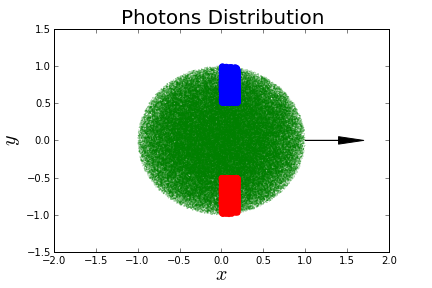
\includegraphics[width=0.40\textwidth]{Distribution.png}
%  \caption{Inhomogeneous distributions of 
% photons, Blue area represents the photons in distribution 1 while red
% area are the selected photons for distribution 2. The arrow points to
% the observer position\label{figure:distributions}}  
%\end{figure}

%In Fig.~\ref{figure:inhomogeneous} we show the resulting spectra of 
%distribution 1 and 2, the first effect we see is the asymmetry of the
%double peak, in the homogeneous and central distribution we see double
%peaks with the same height, while in this case one peak is higher than 
%the other. For $\tau=10^{5}$ we found that in distribution 1 the blueshifted
%peak is higher than the redshifted, and for distribution 2 the redshifted
%peak is the highest.

%An other important fact here is the asymmetry of the spectra with respect 
%to the line center, in particular photons selected in distribution 1 
%present a blueshift in their spectra while photons selected in distribution 
%2 present a redshift. This effect becomes stronger as velocity increase 
%~\ref{figure:inhomogeneous}
 
%\begin{figure*}
%  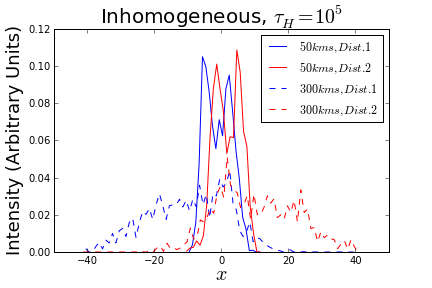
\includegraphics[width=0.45\textwidth]{InomogeneousModelt5.png}
%  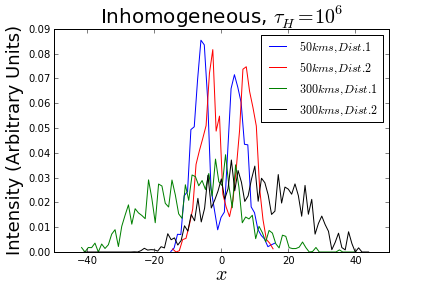
\includegraphics[width=0.45\textwidth]{InomogeneousModelt6.png}
% \caption{Inhomogeneous model for velocities $50km/s$ and $300km/s$ ,
%   (left) with $\tau=10^5$, (right) with
%   $\tau=10^6$\label{figure:inhomogeneous}}  
%\end{figure*}
 

%\subsection{Integrated flux in a narrowband filter}

%Until now we have shown the main effects of gas and dust rotation in
%the Ly$\alpha$ line morphology such as the escape fraction, the FWHM,
%the maxima position, also we see that shape of the outgoing spectra
%depends on the position of the observer. It is important to see if
%rotational effects are detectable in observational methods involving
%the Ly$\alpha$ line.  

%One of the most used methods to detect high redshift galaxies using
%the Ly$\alpha$ line is using a narrowband selection, we make this
%analysis based on the results obtained by Steidel (2011) in this work
%(EXPLAIN a lit of bit more about their work) they used tree narrowband
%filters for tree different redshifts resumed in
%Table~\ref{table:NBfilters}, We want to know how much the integrated
%flux change due to rotational effects in this NB filters, for the
%models we simulated with CLARA. 

%\begin{table*}
%\begin{center}
%\begin{tabular}{cccc}\hline
%Model & SSA22a 4980/80   & HS1549 4667/80 & HS1700 4018/90\\
%\hline
%\end{tabular}
%\caption{
%Fluxes for tree different narrow band filters.
%} 
%\label{table:NBfilters}
%\end{center}
%\end{table*}

%In table \ref{table:NBfilters} we present the results of the flux in
%every  narrowband filter for the homogeneous model at different
%velocities and hydrogen  optical depth $\tau_{0}$. As is well known an
%increase in the optical depth makes  the line peaks separation
%bigger. In fact for some cases the line width is larger  than the NB
%filer width fig.(put ref fig) for those cases we modify the redshift
%in the available range in order to make the peak maxima match the NB
%filter center.  For all cases we found that as velocity increase the
%flux is less.  

%In the case of the dusty model we found the same trend of the flux
%with the velocity  but in this cases the effect is no that strong.  We
%also found some dependency with the viewing angle. 

%\begin{figure}
%  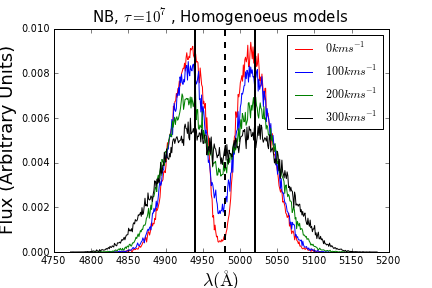
\includegraphics[width=0.45\textwidth]{NB7tDifVHOM.png}
% \label{figure:efvsNeufeld}\caption{NB filter located at the center of
%   the maxima, with different redshift}  
%\end{figure}

\section{Discussion}
\label{sec:discussion}

... Comparison with Verhamme et al. results on the rotation


... Compare with Kulas et al (Figure 3), Rotation on the lyman alpha
line convert double peak profiles into a single one. comments about
rotation with inflows and outflows.   

... The results derived in this paper have consequences on the
interpretation of galaxy observations in the Lyman alpha line.

..compare steidel et al (2011) 


% taking into account equivalent widths results with narrow band
% filters we can make a criterium in order to select wich galaxie
% could be seen in actual observations.  



\section{Conclusions}
In this paper we have estimated the effects of gas bulk rotation on
the emission  of the Lyman $\alpha$ line. We based the study on the
study of a simplified configuration of an homogeneous sphere rotating
as a solid body. We explored  a range of models by varying the
rotation speed, hydrogen optical depth, dust optical depth and initial
distribution of Ly$\alpha$ photons with respect to the gas
density. This was implemented in CLARA, a Monte-Carlo
radiative transfer code already used to study the Lyman $\alpha$
line. 

As first we see how the width of the line changes using a modified FWHM
explained in section \ref{sec:widthpeak}, and we found that as gas bulk 
rotation increase also the width increase in a factor of $2-3$ in comparison 
with the static case. We also take into account the influence of the observer 
viewing angle, we found that observers with a line of sight perpendicular  
to the axis of rotation measure a $15\%$ larger line width than those 
aligned with the rotation axis.

As many observational spectra Ly$\alpha$ emission line (Kulas et al)
is double  peaked, these peaks provide important information
concerning gas kinematics and geometry,  which can be partially
explained with inflows/outflows of gas content.  We study the effect
of rotation in the position of this peaks, and we find  that the
position of the maxima does change with rotation for the homogeneous
models when the double peak merged into a single peak as velocity
increase. This effect is not seen for the central distribution when
the double peak  remains constant as the velocity increase. We also
find that there is no dependency in the observer viewing angle with
the maxima position. 

Concerning the escape fraction under rotational effects on the
Ly$\alpha$ emission line, we found that the escape fraction increase
in about $20\%-30\%$for the homogeneous sphere model. While rotational
effects are negligible for the central models and the escape fraction
remains constant. Also the observer viewing angle have no effect in
the escape fraction neither for the homogeneous and central
models. Complementing this analysis we study the average number of
scatterings $<N_{scatt}>$ that photons perform before escaping of the
cloud taking into account rotational effects. The main result here is
for the homogeneous models for which as velocity increase photons
escape with about $\sim 39\%$  less scatterings than in the static
case. 

As an application of these results we compute the integrated flux
taking into account the narrow band filters used by (Steidel et al
2011), for our models we found an important decrease up to $~40\%$ for
the homogeneous models, and up to $22\%$ for the dusty homogeneous
models in the flux as velocity increase.  Also we calculate at what
redshift should the filter be in order to get the maximum  flux, and
for the tree filters we get values that rely in the filter redshift
range. This effects would have a relevant implication at the time to
find high redshift galaxies.

This paper illustrates for the first time the main effects of rotation
in the morphology of the Ly$\alpha$ emission line, we estimate the
range of this effects for simplified models.


\section*{Acknowledgements}


\bibliography{references} 

\section*{Appendix A: Tables}


\end{document}



%ideas:
Keep in mind making a follow up paper on the results of Yamada et atl
http://adsabs.harvard.edu/abs/2012ApJ...751...29Y on the line
morphology at z=3.1. How many of t hese laes can be considered to have
rotation features? In principle, all of then should have them. How to
make the case convincing in the statistical sense? 

